\documentclass[../informe_krapp.tex]{subfiles}
\begin{document}
\section{Partes del proyecto}
\subsection{El protocolo de comunicación SPI}
\begin{wrapfigure}{r}{0in}
	\centering
	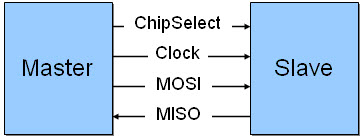
\includegraphics[width= 1.5in, keepaspectratio]{spi-1.jpg}
\end{wrapfigure}

El protocolo Serial Peripheral Interface es un protocolo de comunicación creado por
Motorola, anunciado en el año 1979.
El mismo se divide en 4 lineas de comunicación, cada una con una función específica
(por favor, ver figura \ref{spi-single-slave}) con:

\begin{itemize}
	\item Una señal de clock llamada SCLK, enviada desde el bus master a todos los slaves.
	      Todas las señales del protocolo van as er sínconas a esta señal de clock
	\item Una señal de selección de slave llamada SSn, usada para seleccionar con
	      que slave se esta comunicando el master
	\item Una linea de datos desde master hacia slave, llamada MOSI (Master Out Slave In)
	\item Una linea de datos desde slave hacia master, llamada MISO (Master In Slave OUT)
\end{itemize}

\begin{figure}[H]
	\centering
	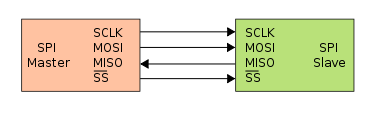
\includegraphics[width=0.5\textwidth]{spi-single-slave.png}
	\caption{SPI master conectado a un único slave.}
	\label{spi-single-slave}
\end{figure}

\begin{figure}[H]
	\centering
	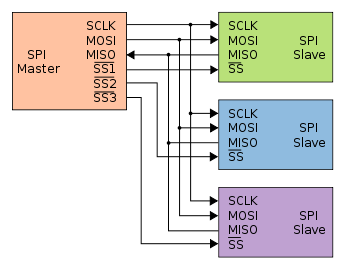
\includegraphics[width=0.5\textwidth]{spi-multiple-slaves.png}
	\caption{SPI master conectado a múltiples slaves.}
	\label{spi-multiple-slaves}
\end{figure}

\todo{no olvidarse de la daisy chained}

\clearpage

SPI es un protoclo de comunicación single-master, esto significa que un dispositivo
central (normalmente un microcontrolador) es el encargado de iniciar todas
las comunicaciónes con los slaves.

Cuando el master SPI desea enviar o recibir información de un slave, selecciona el
slave seteando en LOW la linea SS correspondiente, y activa la señal de clock a una
frecuencia usable por el master y el slave.
A partir de ese momento, el master envía la información por el canal MOSI mientras lee
la información que hay en el canal MISO

\begin{figure}[H]
	\centering
	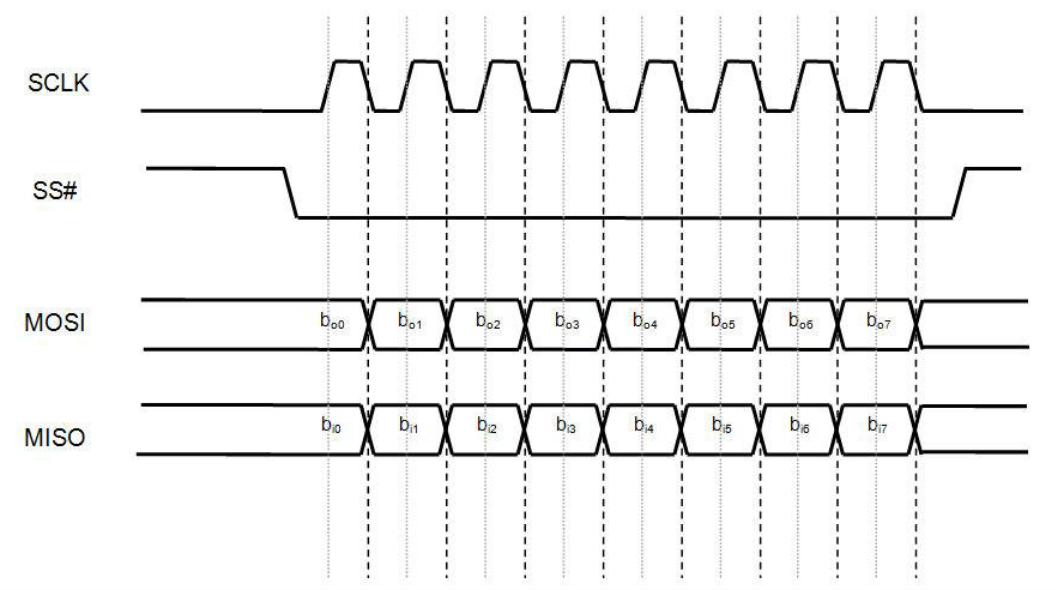
\includegraphics[width=0.7\textwidth]{spi-timing.png}
	\caption{El timing de una comunicación SPI. En este ejemplo,
		La transmisión de datos por los canales MOSI y MISO es ejecutada por
		cada flanco descendente en la señal de clock en SCLK. En cambio,
		la lectura de datos es ejecutada por cada flanco ascendente.
		Esto se puede cambiar modificando el SPI mode }
	\label{spi-timing}
\end{figure}

Como se menciona en la figura \ref{spi-timing}, hay 4 modos SPI, que van del 0 al 3.
Los modos SPI definen en que flanco se activa la linea MOSI, MISO, y el estado (LOW o HIGH)
de inactividad (idle) del canal SCLK.
Cada modo esta definido por un par de parámetros llamados clock polarity
(polaridad de clock) (CPOL), y clock phase (fase de clock) (CPHA)

\begin{figure}[H]
	\centering
	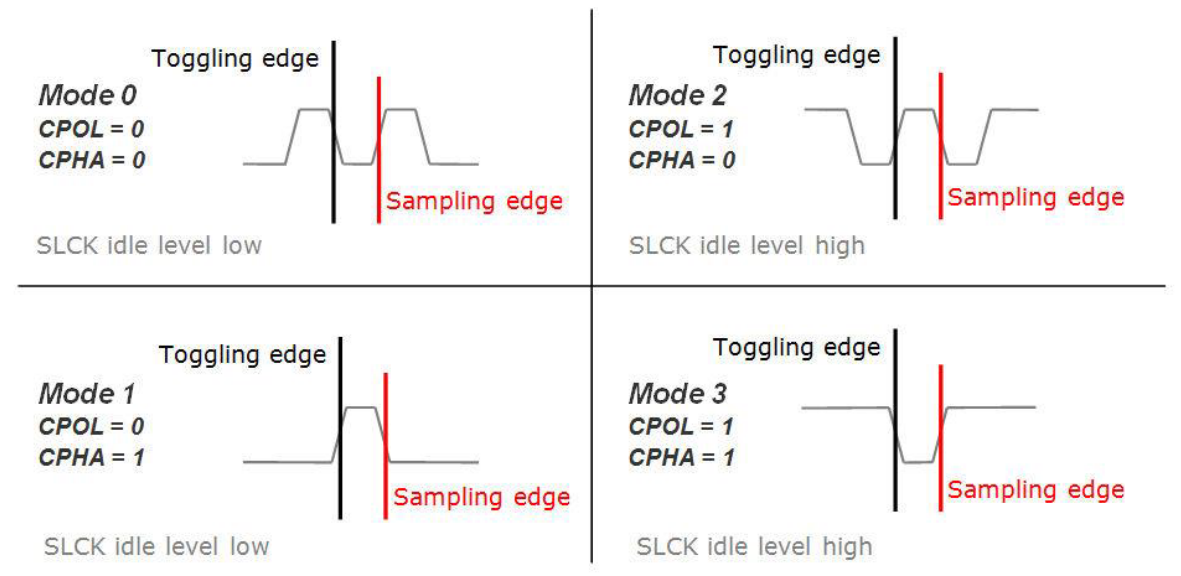
\includegraphics[width=0.7\textwidth]{spi-modes.png}
	\caption{Los modos SPI son definidos con los parámetros CPOL (clock polarity) y CPHA
		(clock phase), que definen 3 parámetros: El flanco usado para envío de datos, el
		flanco usado para recepción de datos, y el estado de inactividad (idle) de SCLK}
	\label{spi-modes}
\end{figure}

Una conexión SPI master/slave tiene que usar el mismo set de parámetros explicados
en la figura \ref{spi-modes} para poder efectuar una comunicación.
Si de todas formas se desea que múltiples slaves tengan configuraciones distintas,
el master deberá reconfigurarse cada vez que se desee comunicar con cada dispositivo.
\begin{figure}[H]
	\centering
	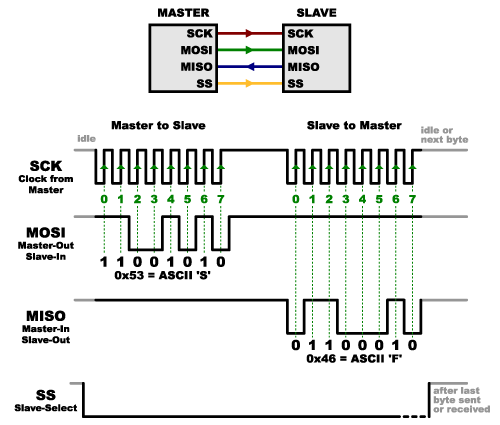
\includegraphics[width=0.7\textwidth]{spi-timing-2.png}
	\caption{Grafico de comunicacion SPI}
\end{figure}

\subsubsection{Ventajas}
Segun Wikipedia\cite{wikipedia_spi}:
\begin{itemize}
	\item Comunicación Full Duplex
	\item Mayor velocidad de transmisión que con I²C o SMBus
	\item Protocolo flexible en que se puede tener un control absoluto sobre los bits transmitidos
	\item No está limitado a la transferencia de bloques de 8 bits
	\item Elección del tamaño de la trama de bits, de su significado y propósito
	\item Su implementación en hardware es extremadamente simple
	\item Consume menos energía que I²C o que SMBus debido que posee menos circuitos (incluyendo las resistencias pull-up) y estos son más simples
	\item No es necesario arbitraje o mecanismo de respuesta ante fallos
	\item Los dispositivos clientes usan el reloj que envía el servidor, no necesitan por tanto su propio reloj
	\item No es obligatorio implementar un transceptor (emisor y receptor), un dispositivo conectado puede configurarse para que solo envíe, sólo reciba o ambas cosas a la vez
	\item Usa mucho menos terminales en cada chip/conector que una interfaz paralelo equivalente
	\item Como mucho una única señal específica para cada cliente (señal SS), las demás señales pueden ser compartidas
\end{itemize}

\subsubsection{Desventajas}
\begin{itemize}
	\item Consume más pines de cada chip que I²C, incluso en la variante de 3 hilos
	\item El direccionamiento se hace mediante líneas específicas (señalización fuera de banda) a diferencia de lo que ocurre en I²C que se selecciona cada chip mediante una dirección de 7 bits que se envía por las mismas líneas del bus
	\item No hay control de flujo por hardware
	\item No hay señal de asentimiento. El servidor podría estar enviando información sin que estuviese conectado ningún cliente y no se daría cuenta de nada
	\item No permite fácilmente tener varios servidores conectados al bus
	\item Sólo funciona en las distancias cortas a diferencia de, por ejemplo, RS-232, RS-485, o Bus CAN
\end{itemize}







\clearpage

\subsection{DOIT ESP32 DevKit v1}
\begin{wrapfigure}{r}{0in}
	\centering
	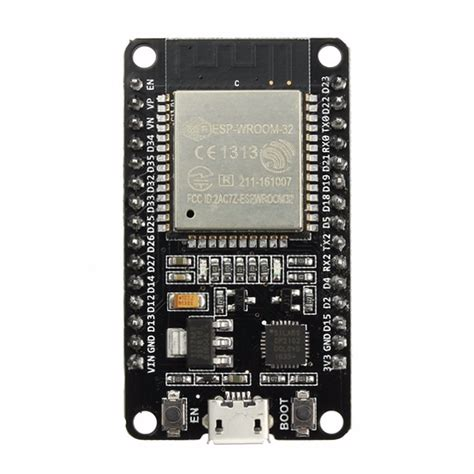
\includegraphics[width= 1.5in, keepaspectratio]{ESP32-board.jpg}
\end{wrapfigure}
El kit de desarrollo DOIT ESP32 DevKit v1 es una de las placas de desarrollo creadas por
DOIT. Esta basada en el microcontrolador ESP32, que en un mismo chip tiene soporte
para WiFi, Bluetooth, Ethernet y Low-Power

\subsubsection{Características Técnicas}
\begin{itemize}
	\item Microcontrolador: Tensilica 32-bit Single/Dual-core CPU Xtensa LX6
	\item Tensión de operación: 3.3V
	\item Tensión de alimentación: 7-12V
	\item Pines I/O digitales (DIO): 25
	\item Pines analógicos de Entrada (ADC): 6
	\item Pines analógicos de Salida (DAC): 2
	\item UARTs: 3
	\item SPIs: 2
	\item I2Cs: 3
	\item Memoria Flash: 4 MB
	\item SRAM: 520 KB
	\item Velocidad de clock: 240 Mhz
	\item Wi-Fi: IEEE 802.11 b/g/n/e/i, con las siguientes características:
	      \begin{itemize}
		      \item Switch TR, Balun, LNA, Amplificador de potencia y antena integrados
		      \item Autenticación WEP, WPA/WPA2, con la opcion de tambien acceder a redes abiertas.
	      \end{itemize}
\end{itemize}

\clearpage

\subsubsection{Pinout}
\begin{figure}[H]
	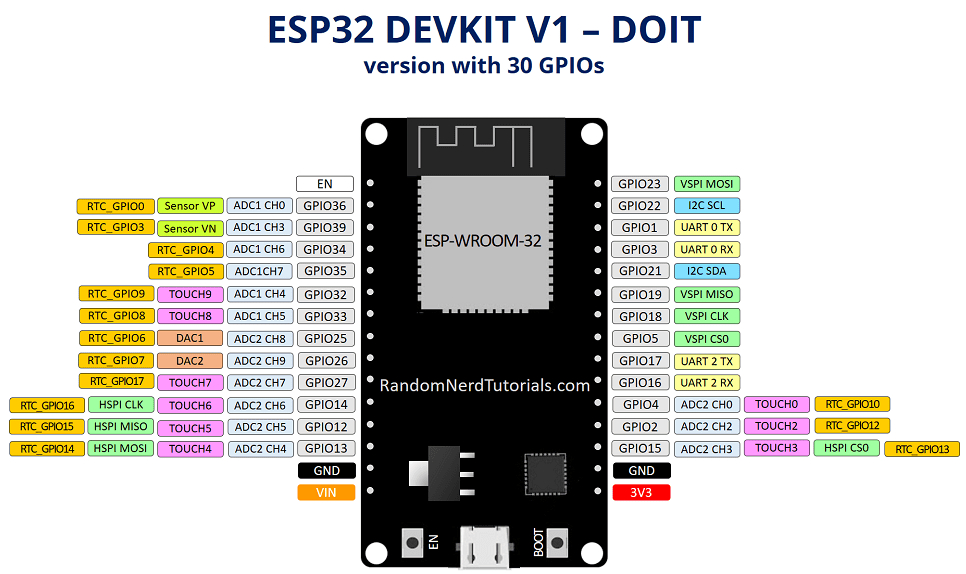
\includegraphics[width=0.85\textwidth]{ESP32-board-30pin-pinout.jpg}
	\centering
	\caption{Pinout de la placa de desarrollo DOIT DevKit V1 ESP32 de 30 pines}
\end{figure}

\begin{figure}[H]
	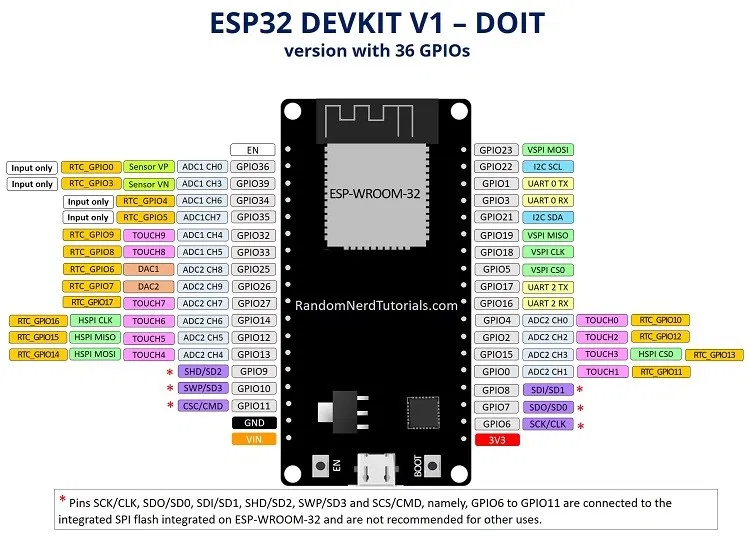
\includegraphics[width=0.85\textwidth]{ESP32-board-36pin-pinout.jpg}
	\centering
	\caption{Pinout de la placa de desarrollo DOIT DevKit V1 ESP32 de 36 pines,
		cabe recordar que los pines GPIO 6-11 estan reservados al sistema SPI integrado, y su
		uso no es recomendado}
\end{figure}
\subsubsection{Usabilidad de pines}
El ESP32 cuenta con una multitud de pines, pero no todos pueden ser usados libremente,
esto es explicado en la tabla \ref{tabla-pines-esp32} que muestra que pines pueden ser utilizados y cuales no,
dependiendo de las cirscuntancias.

A la hora de ser usados en el codigo c++ del framework Arduino, simplemente se refieren
por el numero

\begin{table}[!ht]
	\centering
	\begin{tabular}{|l|l|l|l|}
		\hline
		GPIO & Input     & Output & Notes                                      \\ \hline
		0    & pulled up & OK     & Hace output de señal PWM al arranque       \\ \hline
		1    & TX pin    & OK     & debug output al arranque                   \\ \hline
		2    & OK        & OK     & Conectado al LED\_ONBOARD                  \\ \hline
		3    & OK        & RX pin & En estado HIGH al arranque                 \\ \hline
		4    & OK        & OK     & ~                                          \\ \hline
		5    & OK        & OK     & Hace output de señal PWM al arranque       \\ \hline
		6    & x         & x      & Conectado al flash SPI integrado           \\ \hline
		7    & x         & x      & Conectado al flash SPI integrado           \\ \hline
		8    & x         & x      & Conectado al flash SPI integrado           \\ \hline
		9    & x         & x      & Conectado al flash SPI integrado           \\ \hline
		10   & x         & x      & Conectado al flash SPI integrado           \\ \hline
		11   & x         & x      & Conectado al flash SPI integrado           \\ \hline
		12   & OK        & OK     & El arranque falla si está pulleado en HIGH \\ \hline
		13   & OK        & OK     & ~                                          \\ \hline
		14   & OK        & OK     & Hace output de señal PWM al arranque       \\ \hline
		15   & OK        & OK     & Hace output de señal PWM al arranque       \\ \hline
		16   & OK        & OK     & ~                                          \\ \hline
		17   & OK        & OK     & ~                                          \\ \hline
		18   & OK        & OK     & ~                                          \\ \hline
		19   & OK        & OK     & ~                                          \\ \hline
		21   & OK        & OK     & ~                                          \\ \hline
		22   & OK        & OK     & ~                                          \\ \hline
		23   & OK        & OK     & ~                                          \\ \hline
		25   & OK        & OK     & ~                                          \\ \hline
		26   & OK        & OK     & ~                                          \\ \hline
		27   & OK        & OK     & ~                                          \\ \hline
		32   & OK        & OK     & ~                                          \\ \hline
		33   & OK        & OK     & ~                                          \\ \hline
		34   & OK        & x      & Solamente de input                         \\ \hline
		35   & OK        & x      & Solamente de input                         \\ \hline
		36   & OK        & x      & Solamente de input                         \\ \hline
		39   & OK        & x      & Solamente de input                         \\ \hline
	\end{tabular}
	\caption{Una tabla con las funciones de cada pin de la placa de desarrollo
		DOIT DevKit v1 ESP32}
	\label{tabla-pines-esp32}
\end{table}





\clearpage
\subsection{Sistema RFID}
Segun Wikipedia\cite{wikipedia_rfid_es}:

\begin{center}
	\rule{0.8\textwidth}{0.3pt}
\end{center}
``RFID o identificación por radiofrecuencia
(del inglés Radio Frequency Identification) es un sistema de almacenamiento y recuperación
de datos remotos que usa dispositivos denominados etiquetas, tarjetas o transpondedores
RFID.

\begin{wrapfigure}{r}{0in}
	\centering
	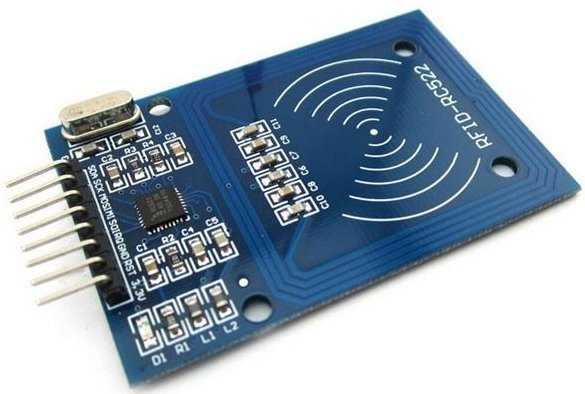
\includegraphics[width= 1.5in, keepaspectratio]{rfid-rc552.jpg}
\end{wrapfigure}

El propósito fundamental de la tecnología RFID es transmitir la identidad de
un objeto (similar a un número de serie único) mediante ondas de radio. Las tecnologías
RFID se agrupan dentro de las denominadas Auto ID (automatic identification,
o identificación automática).

Las etiquetas RFID (RFID tag en inglés) son unos dispositivos pequeños, similares
a una pegatina, que pueden ser adheridas o incorporadas a un producto, un animal
o una persona. Contienen antenas para permitirles recibir y responder a peticiones
por radiofrecuencia desde un emisor-receptor RFID. Las etiquetas pasivas no necesitan
alimentación eléctrica interna, mientras que las activas sí lo requieren.

Una de las ventajas del uso de radiofrecuencia (en lugar, por ejemplo, de infrarrojos)
es que no se requiere visión directa entre emisor y receptor''

\begin{center}
	\rule{0.8\textwidth}{0.3pt}
\end{center}

\begin{figure}[H]
	\centering
	\begin{subfigure}{0.4\textwidth}
		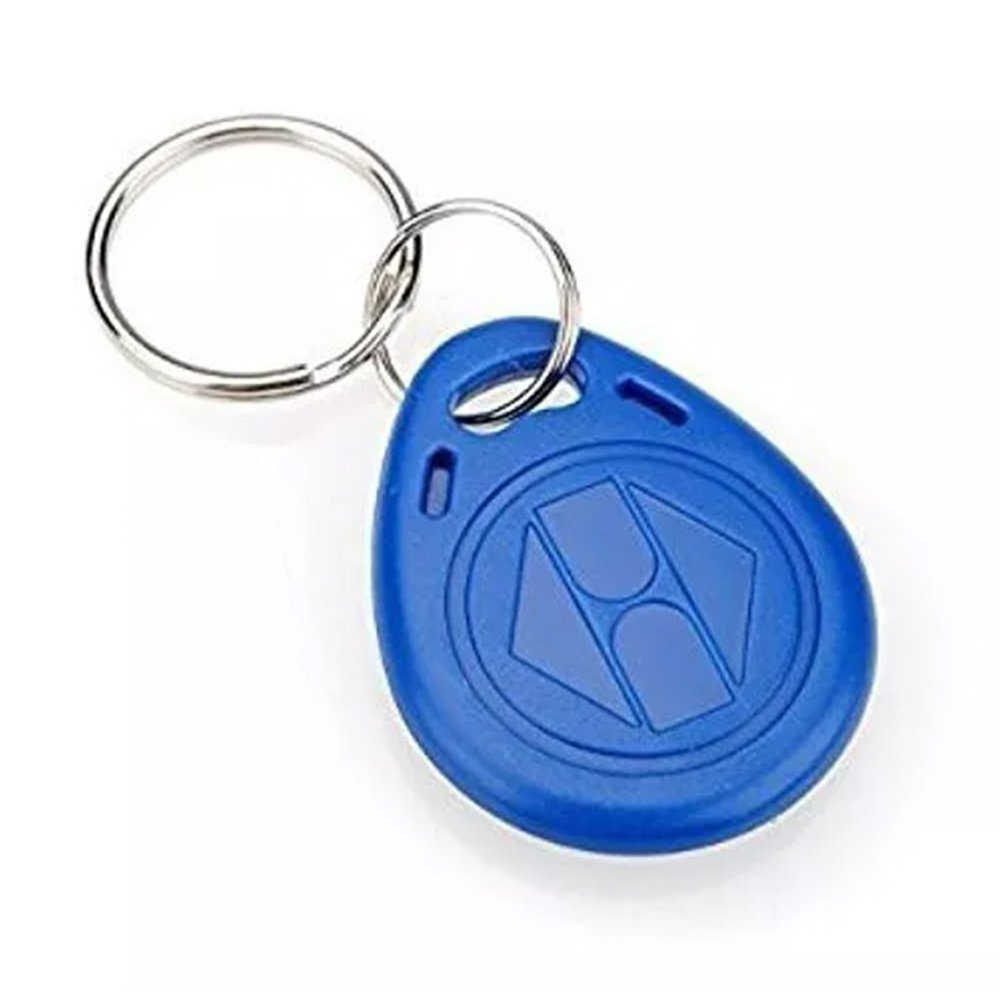
\includegraphics[width=0.7\textwidth]{llavero-rfid.jpg}
		\caption{Un llavero RFID}
	\end{subfigure}
	\begin{subfigure}{0.4\textwidth}
		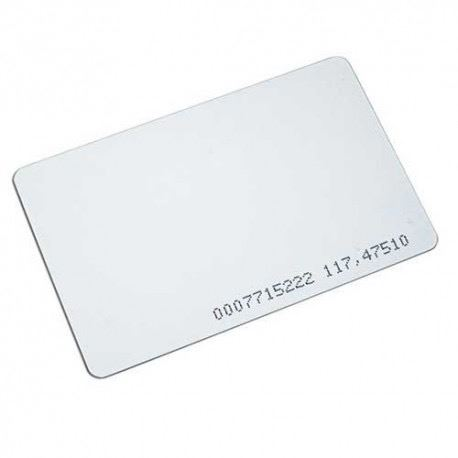
\includegraphics[width=0.7\textwidth]{tarjeta-rfid.jpg}
		\caption{Una tarjeta RFID}
	\end{subfigure}
	\caption{Distintos tags RFID}
\end{figure}

\clearpage
\subsubsection{Pinout del dispositivo}

\begin{wrapfigure}{r}{0in}
	\centering
	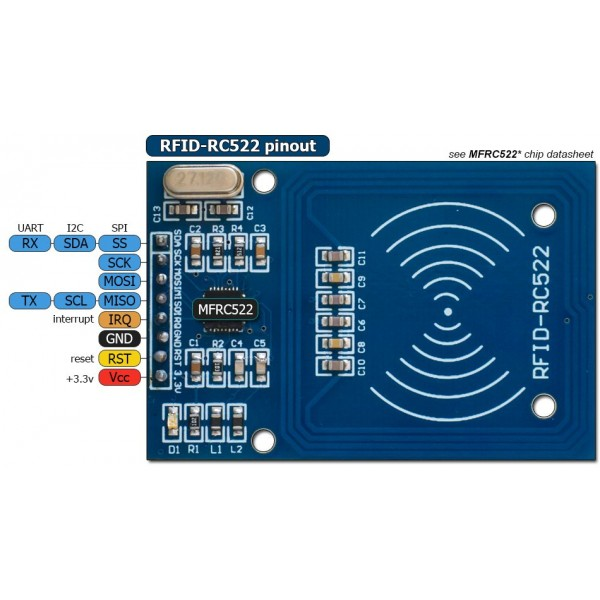
\includegraphics[width=0.5\textwidth]{rfid-rc522-pinout.jpg}
	\caption{El pinout del lector RFID-RC552.
		Se puede notar como este dispositivo está adaptado para funcionar con 3 protocolos
		distintos, comunicación por UART, comunicación por I2C y comunicacion por SPI}
\end{wrapfigure}

% la verdad es que este "---" esta RE mal, lo tendria que cambiar con titlesec

\paragraph{pin SDA ---}
Este pin se utiliza de forma distinta dependiendo del protocolo
de comunicación utilizado.
\begin{itemize}
	\item En I2C, se usa como el pin SDA.
	\item En UART, se usa como pin RX.
	\item En SPI, se usa como el pin SS
\end{itemize}

\paragraph{pin SCK ---}
El pin SCK se usa para mantener el sincronísmo con una señal de reloj

\paragraph{pin MOSI ---}
El pin MOSI sirve para hacer una transmisión Master Out - Slave In

\paragraph{pin MISO ---}
El pin MISO sirve para hacer una transmisión Master In - Slave Out

\paragraph{pin IRQ ---}
Se usa para las interrupciones

\paragraph{GND ---}
Sirve para mantener la referencia con Masa

\paragraph{RST ---}
Este pin sirve para resetear o desactivar el circuito integrado

\paragraph{VCC ---}
Pin de alimentación \textbf{3.3v}

\clearpage
\subsubsection{Mapeo de Memoria del tag RFID}
La identificación se realiza con unos llaveros o unas tarjetas,
que tienen este mapeo de memoria:

Tenemos 1k de memoria adentro de este chip, la cual esta organizada de la
siguiente manera: Hay 16 sectores de 4 bloques, y cada bloque contiene 16 bytes.

\begin{figure}[H]
	\centering
	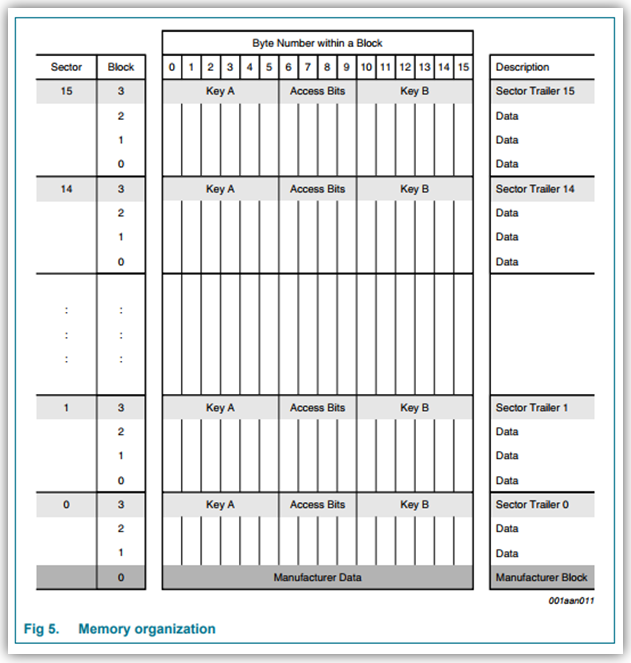
\includegraphics[width=0.7\textwidth]{rfid-mapeo-memoria.png}
\end{figure}

\subsection{Frameworks y demás}
\subsubsection{Arduino}
Para este proyecto, se uso el framework Arduino, que provee una amplia variedad de
clases, metodos y funciones útiles para el desarrollo en sistemas embebidos.

Este framework se implementó a través de platformIO, una extensión de Visual Studio Code.

En este proyecto, todo el desarrollo del ESP32 fue hecho mediante este framework.

\subsubsection{Flask}
Flask es un microframework usado para crear aplicaciones webs. Este, al ser modular y escalable, tiene la posibilidad
de permitir el agregado de ORM's (Object Relational Manager), routers, renderizador de templates, sistema de logins,
sistema de Forms, etc...

En este proyecto, Flask se usó para el desarrollo del backend, incluyendo la API.

\subsubsection{Bootstrap}

Bootstrap es el framework CSS más popular para desarrollar aplicaciones responsivas y aptas para dispositivos móviles.

En este proyecto, Bootstrap se usó la versión 5 para el desarrollo del frontend.

\subsubsection{Amazon Web Services (AWS)}

Amazon Web Services (AWS) es la plataforma cloud más adoptada en el mundo, con más de 200 servicios distintos.

En este proyecto, AWS se usó para la implementación de la infrastructura de la webapp.
Se usarón los servicios de Relational Database Service (RDS) y Elastic Beanstalk.

\begin{comment}

Segun la referencia de Arduino\cite{arduino_reference}, estas son las cosas que
el framework provee:

\begin{multicols}{2}
	[
		\subsubsection{Funciones}
		Para controlar la placa y realizar cómputos
	]
	\paragraph{Digital I/O}
	\begin{itemize}
		\item digitalRead()
		\item digitalWrite()
		\item pinMode()
	\end{itemize}

	\paragraph{Analog I/O}
	\begin{itemize}
		\item analogRead()
		\item analogReference()
		\item analogWrite()
	\end{itemize}

	\paragraph{Zero, Due \& MKR Family}
	\begin{itemize}
		\item analogReadResolution()
		\item analogWriteResolution()
	\end{itemize}

	\paragraph{Advanced I/O}
	\begin{itemize}
		\item noTone()
		\item pulseIn()
		\item pulseInLong()
		\item shiftIn()
		\item shiftOut()
		\item tone()
	\end{itemize}

	\paragraph{Time}
	\begin{itemize}
		\item delay()
		\item delayMicroseconds()
		\item micros()
		\item millis()
	\end{itemize}

	\paragraph{Math}
	\begin{itemize}
		\item abs()
		\item constrain()
		\item map()
		\item max()
		\item min()
		\item pow()
		\item sq()
		\item sqrt()
	\end{itemize}

	\paragraph{Trigonometry}
	\begin{itemize}
		\item cos()
		\item sin()
		\item tan()
	\end{itemize}

	\paragraph{Characters}
	\begin{itemize}
		\item isAlpha()
		\item isAlphaNumeric()
		\item isAscii()
		\item isControl()
		\item isDigit()
		\item isGraph()
		\item isHexadecimalDigit()
		\item isLowerCase()
		\item isPrintable()
		\item isPunct()
		\item isSpace()
		\item isUpperCase()
		\item isWhitespace()
	\end{itemize}

	\paragraph{Random Numbers}
	\begin{itemize}
		\item random()
		\item randomSeed()
	\end{itemize}

	\paragraph{Bits and Bytes}
	\begin{itemize}
		\item bit()
		\item bitClear()
		\item bitRead()
		\item bitSet()
		\item bitWrite()
		\item highByte()
		\item lowByte()
	\end{itemize}

	\paragraph{External Interrupts}
	\begin{itemize}
		\item attachInterrupt()
		\item detachInterrupt()
	\end{itemize}

	\paragraph{Interrupts}
	\begin{itemize}
		\item interrupts()
		\item noInterrupts()
	\end{itemize}

	\paragraph{Communication}
	\begin{itemize}
		\item Serial
		\item SPI
		\item Stream
		\item Wire
	\end{itemize}

	\paragraph{USB}
	\begin{itemize}
		\item Keyboard
		\item Mouse
	\end{itemize}
\end{multicols}

\clearpage

\begin{multicols}{2}
	[
		\subsubsection{Variables}
		Tipos de Datos y Constantes definidos en el framework
	]
	\paragraph{Constants}
	\begin{itemize}
		\item HIGH | LOW
		\item INPUT | OUTPUT | INPUT\_PULLUP
		\item LED\_BUILTIN
		\item true | false
		\item Floating Point Constants
		\item Integer Constants
	\end{itemize}

	\paragraph{Conversion}
	\begin{itemize}
		\item (unsigned int)
		\item (unsigned long)
		\item byte()
		\item char()
		\item float()
		\item int()
		\item long()
		\item word()
	\end{itemize}

	\paragraph{Data Types}
	\begin{itemize}
		\item array
		\item bool
		\item boolean
		\item byte
		\item char
		\item double
		\item float
		\item int
		\item long
		\item short
		\item size\_t
		\item string
		\item String()
		\item unsigned char
		\item unsigned int
		\item unsigned long
		\item void
		\item word
	\end{itemize}

	\paragraph{Variable Scope \& Qualifiers}
	\begin{itemize}
		\item const
		\item scope
		\item static
		\item volatile
	\end{itemize}

	\paragraph{Utilities}
	\begin{itemize}
		\item PROGMEM
		\item sizeof()
	\end{itemize}
\end{multicols}

\clearpage

\begin{multicols}{2}
	[
		\subsubsection{Estructura}
		Los elementos del codigo Arduino (C++).
	]
	\paragraph{Sketch}
	\begin{itemize}
		\item loop()
		\item setup()
	\end{itemize}

	\paragraph{Control Structure}
	\begin{itemize}
		\item break
		\item continue
		\item do...while
		\item else
		\item for
		\item goto
		\item if
		\item return
		\item switch...case
		\item while
	\end{itemize}

	\paragraph{Further Syntax}
	\begin{itemize}
		\item \#define (define)
		\item \#include (include)
		\item /* */ (block comment)
		\item // (single line comment)
		\item ; (semicolon)
		\item {} (curly braces)
	\end{itemize}

	\paragraph{Arithmetic Operators}
	\begin{itemize}
		\item \% (remainder)
		\item * (multiplication)
		\item + (addition)
		\item - (subtraction)
		\item / (division)
		\item = (assignment operator)
	\end{itemize}

	\paragraph{Comparison Operators}
	\begin{itemize}
		\item != (not equal to)
		\item < (less than)
		\item <= (less than or equal to)
		\item == (equal to)
		\item > (greater than)
		\item >= (greater than or equal to)
	\end{itemize}

	\paragraph{Boolean Operators}
	\begin{itemize}
		\item ! (logical not)
		\item \&\& (logical and)
		\item || (logical or)
	\end{itemize}

	\paragraph{Pointer Access Operators}
	\begin{itemize}
		\item \& (reference operator)
		\item * (dereference operator)
	\end{itemize}

	\paragraph{Bitwise Operators}
	\begin{itemize}
		\item \& (bitwise and)
		\item <~<~ (bitshift left)
		\item >~>~ (bitshift right)
		\item \^ ~ (bitwise xor)
		\item | (bitwise or)
		\item \~~ (bitwise not)
	\end{itemize}

	\paragraph{Compound Operators}
	\begin{itemize}
		\item \%= (compound remainder)
		\item \&= (compound bitwise and)
		\item *= (compound multiplication)
		\item ++ (increment)
		\item += (compound addition)
		\item -~- (decrement)
		\item -~= (compound subtraction)
		\item /= (compound division)
		\item \^~= (compound bitwise xor)
		\item |= (compound bitwise or)
	\end{itemize}
	
\end{multicols}
\end{comment}
\end{document}